\section{Redes de Computadores}
    Tanenbaum em \textit{Redes de Computadores} define um sistema distribuído como sendo um: %(TANENBAUM, Andrew S. Redes de Computadores. Tradução da 4rd. Ed. em inglês. Editora Campus. 2003.)

    \begin{quote}
        ``Conjunto de computadores autônomos interconectados por uma única tecnologia.''
     \end{quote}

    O que leva a uma errada compreensão de que uma rede de computadores é um sistema distribuído e vice-versa. De fato eles são bastantes semelhantes, mas a diferença se dá que, em um sistema distribuído, o middleware implementa um único modelo que é apresentado ao usuário, portanto um conjunto de computadores independentes passa a impressão de um único sistema coerente. Já em uma rede de computadores, o middleware não está presente fazendo com que esse modelo único também não exista, expondo ao usuário as máquinas reais, deixando claro que ele está lidando com um sistema heterogêneo que possui componentes e sistemas operacionais diferentes.

    Quando se tem um middleware instalado em uma rede, trata-se de um sistema distribuído. Pode-se dizer então que um sistema distribuído é um sistema de software instalado em uma rede. Portanto, a nível de hardware, um SD e uma rede são a mesma coisa e fica sob responsabilidade do sistema operacional determinar a diferença entre um sistema distribuído e uma rede.

    Para que tudo funcione perfeitamente, uma rede precisa ter conjunto de regras que regem a comunicação entre dois ou mais hosts, esse conjunto de regras é chamado de protocolos.%(file:///home/marco/Downloads/pdfcoffee.com_mohammed-m-alani-guide-to-osi-and-tcpip-models-pdf-free.pdf)

    \subsection{Modelo em camadas}
        Para padronização e melhor entendimento da operação de uma rede de computadores foi criado um modelo baseado em camadas. Esse modelo divide em camadas as regras (protocolos) que precisam acontecer para que haja a interconectividade entre dois sistemas, o que facilita a implementação de uma rede pois cada camada tem seus protocolos específicos e bem definidos, fazendo com que esses protocolos consigam executar suas funções de forma mais eficiente. Com essa separação também fica mais fácil de resolver eventuais problemas, visto que se torna possível isolar cada camada sem que seja necessário mexer na rede como um todo.

        \subsection{Open Systems Interconnection (OSI)}
            Este modelo foi proposto por um grupo da Honeywell Information Systems, liderado por Mike Canepa e publicado na década de 70 pela International Organization for Standardization (ISO). Ele é baseado em 7 camadas, cada camada é responsável por fazer uma parte do processo necessário para que duas máquinas se comuniquem. Essas camadas possuem uma hierarquia, fazendo com que cada camada só possa se comunicar com a camada que está imediatamente acima ou abaixo dela.  Cada camada trata seus dados de uma maneira específica, de modo que cada uma é capaz de adicionar novos dados aos dados resultantes da camada anterior, processo chamado de encapsulamento, e esses dados tratados recebem o nome de Protocol Data Unit (PDU).

		    Este modelo possui uma estratégia de camada em pares, o que significa dizer que cada informação adicionada em uma camada pelo lado do emissor deve chegar à camada de mesmo nível do lado do receptor.

		    Na imagem \ref{fig:modelo-osi} está representada as 7 camadas do modelo OSI que estão dispostas da seguinte maneira:

        \begin{itemize}
            \item \textbf{Física:} Estabelece a comunicação real entre os dispositivos;
            \item \textbf{Enlace:} Detecção e correção de erros que aconteceu na camada anterior, controle de fluxo  da transmissão de dados entre dispositivos;
            \item \textbf{Rede:} Endereçamento dos dispositivos na rede, caminho que as informações deverão seguir da origem até o destino (roteamento);
            \item \textbf{Transporte:} Detecção e correção de erros das camadas inferiores, controle de fluxo de dados da origem até o destino e ordenação para garantir que os dados cheguem da mesma forma que foram enviados;
            \item \textbf{Sessão:} Comunicação entre processos dos diferentes sistemas;
            \item \textbf{Apresentação:} Conversão dos formatos de caractere para serem usados na transmissão, compressão e criptografia;
            \item \textbf{Aplicação:} Programas de computadores tanto dos servidores quanto dos clientes;
        \end{itemize}

        \begin{figure}[h]
          \centering
          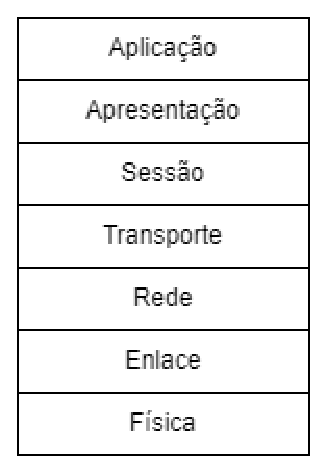
\includegraphics[width=0.8\textwidth]{figuras/modelo-osi.eps}
          \caption{Sistema distribuído organizado como middleware - Imagem retirada de \cite{}.}
          \label{fig:modelo-osi}
        \end{figure}
          

        \subsection{Pilha TCP/IP}
            O modelo OSI é um modelo de referência, mas na prática a internet está modelada de outra forma. A modelagem da internet atualmente
    % \subsection{ethernet (enlace)}
    % \subsection{ipv4 (rede)}
    % \subsection{ipv6 (rede)}
    % \subsection{tcp/ip (transporte)}
    % \subsection{capítulo 6 pra frente}
    % \subsection{topologia de redes}
    % \subsection{modelagem de uma topologia de rede}